\chapter{Transient Noise Detection}\label{ch:TransientNoiseDetection}

\ifpdf
    \graphicspath{{Chapter5_TransNoiseDet/Chapter5Figs/PNG/}{Chapter5_TransNoiseDet/Chapter5Figs/PDF/}{Chapter5_TransNoiseDet/Chapter5Figs/}}
\else
    \graphicspath{{Chapter5_TransNoiseDet/Chapter5Figs/EPS/}{Chapter5_TransNoiseDet/Chapter5Figs/}}
\fi

The rapid increase in availability of high speed internet connections has made personal computers a popular basis for teleconferencing applications. While embedded microphones, loudspeakers and webcams in laptop computers have made setting up conference calls very easy, it has also brought with it some specific noise difficulties such as feedback, fan noise and button clicking noise. The latter has been a particularly persistent problem and is generally due to the mechanical impulses caused by keystrokes. Particularly on laptop computers this can be a significant nuisance due to the mechanical connection between microphone, within in the laptop case, and the keyboard. The noise pulses produced can vary greatly with factors such as keystroke speed and length, microphone placement and response, laptop frame or base, keyboard or trackpad type and even surface on which the computer is placed.

As noted in the literature review, chapter~\ref{sec:LitRev_Detection}, a range of approaches has been taken to detect impulsive noise in speech and audio. In general the approaches taken can be divided into two categories. The ones that focus on corruptions caused by mechanical defects in the medium or errors in the communication channel and 

\section{A look at the data}
\subsection{Spectral investigation of audio signals}
Figure~\ref{fig:spectrogramMarkedTapsBrownFox} shows a spectrogram of a short sequence of speech with typing strokes embedded in it. The figure overlays show the approximate positions of the strokes in the spectrogram. It can be observed that the typing strokes have a fairly flat frequency response compered to the the voiced parts of the audio sequence.

\begin{figure}[!] %spectrogramMarkedTapsBrownFox
\centering
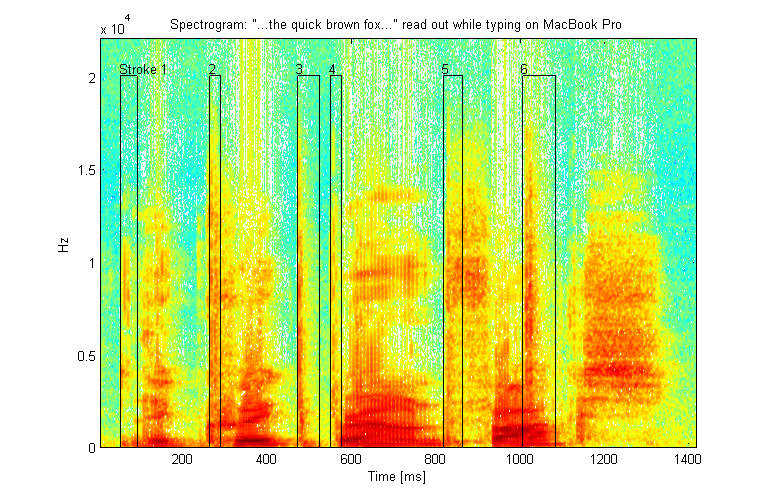
\includegraphics[width=150mm]{spectrogramMarkedTapsBrownFox.png}
\caption{Spectrogram analysis of mixed typing strokes and speech. Overlay shows positions of typing strokes.}\label{fig:spectrogramMarkedTapsBrownFox}
\end{figure}

Figure~\ref{fig:waveletspectrumAno} shows the wavelet spectrum of a sequence of keystrokes with speech interference. The figure overlays show the approximate positions of the strokes in the wavelet spectrum.
\begin{figure}[!] %waveletspectrumAno
\centering
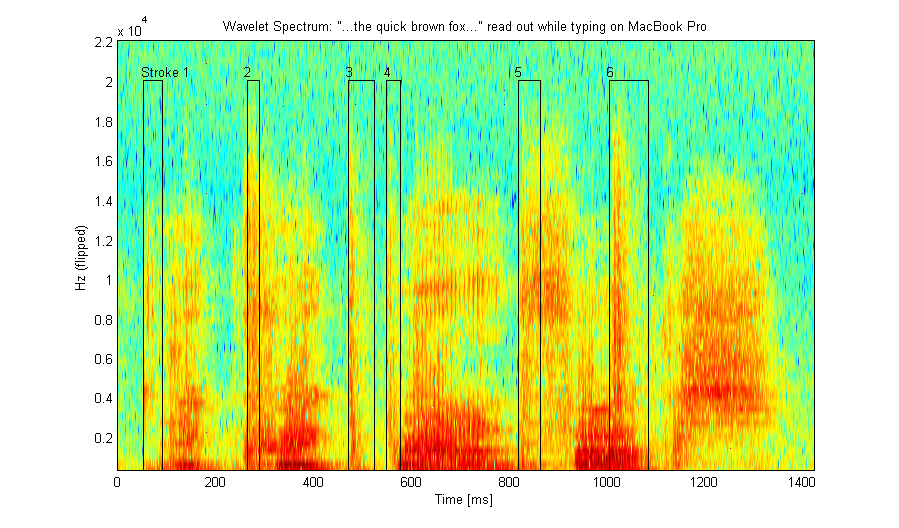
\includegraphics[width=150mm]{waveletspectrumAno.png}
\caption{Top: Waveform of typing sequence. Bottom: Wavelet spectrum of same typing sequence.}\label{fig:waveletspectrumAno}
\end{figure}

\subsection{Keystroke sequence investigation}
A single keystroke, during rapid typing and not at the end of a typing sequence, is generally made up of 3 primary sections.
\begin{enumerate}
  \item A primary \textbf{Stroke} keystroke (15 - 40 ms),
  \item a \textbf{Break} while key is depressed (50 - 500 ms) and
  \item a \textbf{Lift} impulse (15 - 40 ms).
\end{enumerate}
The duration of the break region will typically be determined by the typing speed of the user while the Stroke and the Lift region are primarily constant and will vary more with factors such as stroking force and the vibrational characteristics of the keyboard and the laptop casing.

Figure~\ref{fig:KeyboardStrokeSlow} shows a waveform of a single typing stroke. The waveform clearly shows the two distinct impulses of sudden erratic excitation followed by a slowly decaying low frequency sinusoid.

\begin{figure}[!] %KeyboardStrokeSlow
\centering
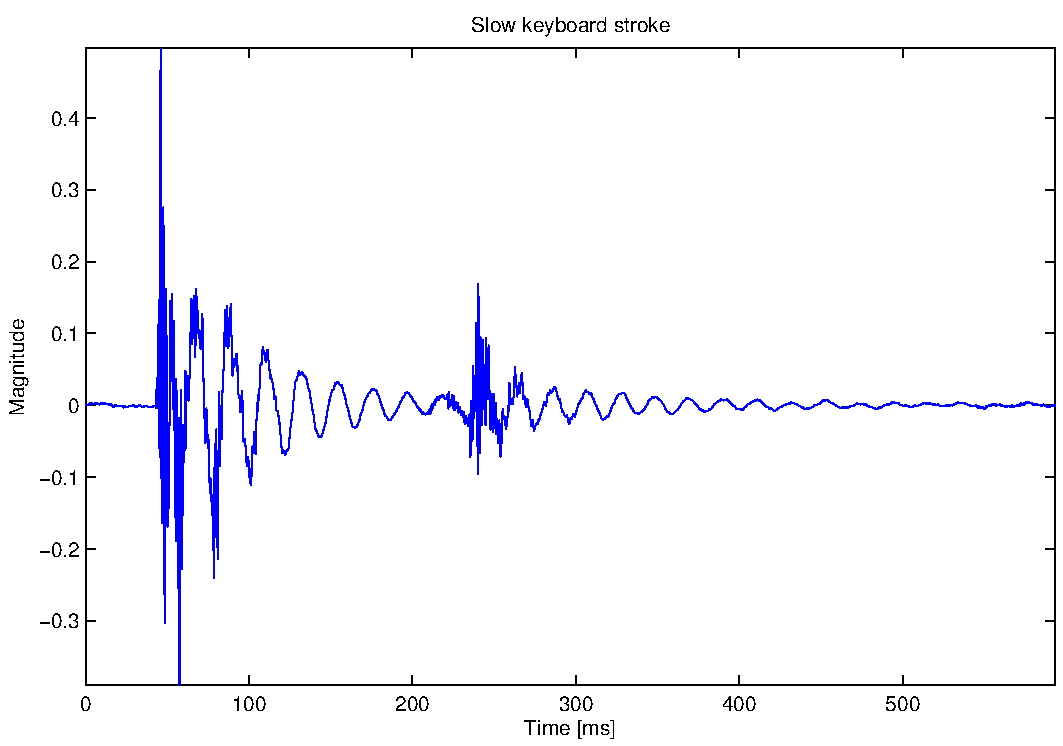
\includegraphics[width=120mm]{KeyboardStrokeSlow.pdf}
\caption{Single slow keyboard stroke.}\label{fig:KeyboardStrokeSlow}
\end{figure}

Figure~\ref{fig:Keyboard2StrokesFast} shows a sequence of two keystrokes in rapid succession. The keystroke regions mentioned above are clearly annotated with their temporal extent also noted.

\begin{figure}[!] %Keyboard2StrokesFast
\centering
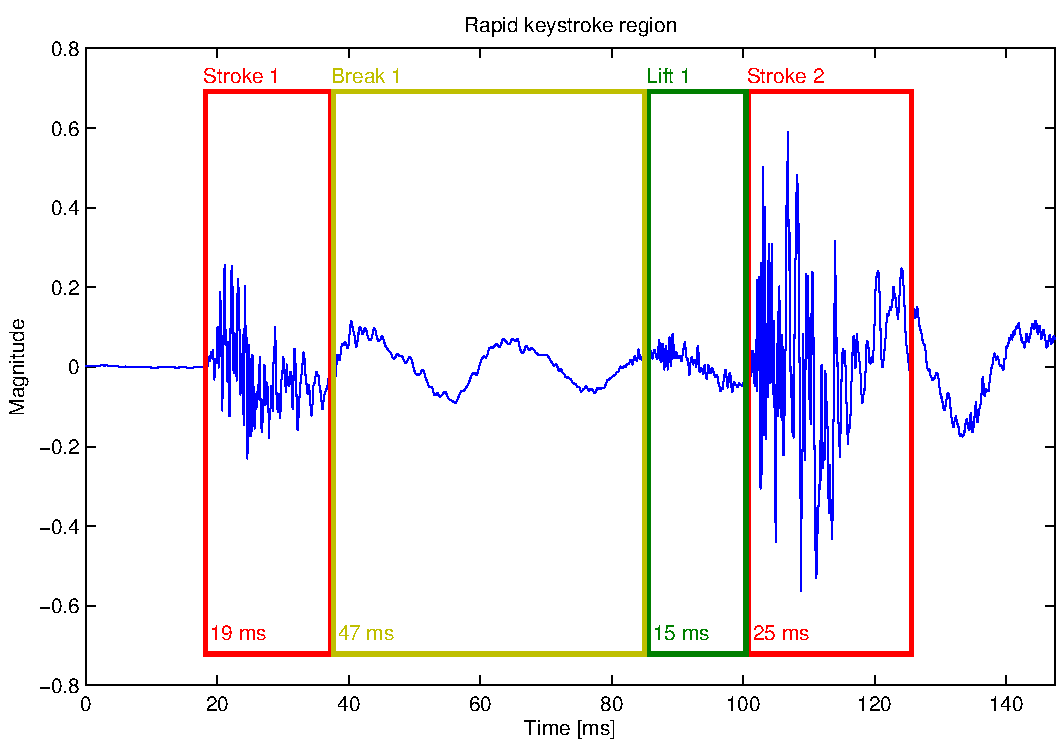
\includegraphics[width=120mm]{Keyboard2StrokesFast.pdf}
\caption{Two annotated keyboard strokes in rapid succession.}\label{fig:Keyboard2StrokesFast}
\end{figure}

Figure~\ref{fig:Keyboard4StrokesFast} shows an example of a short rapid 4 keystroke sequence.

\begin{figure}[!] %Keyboard4StrokesFast
\centering
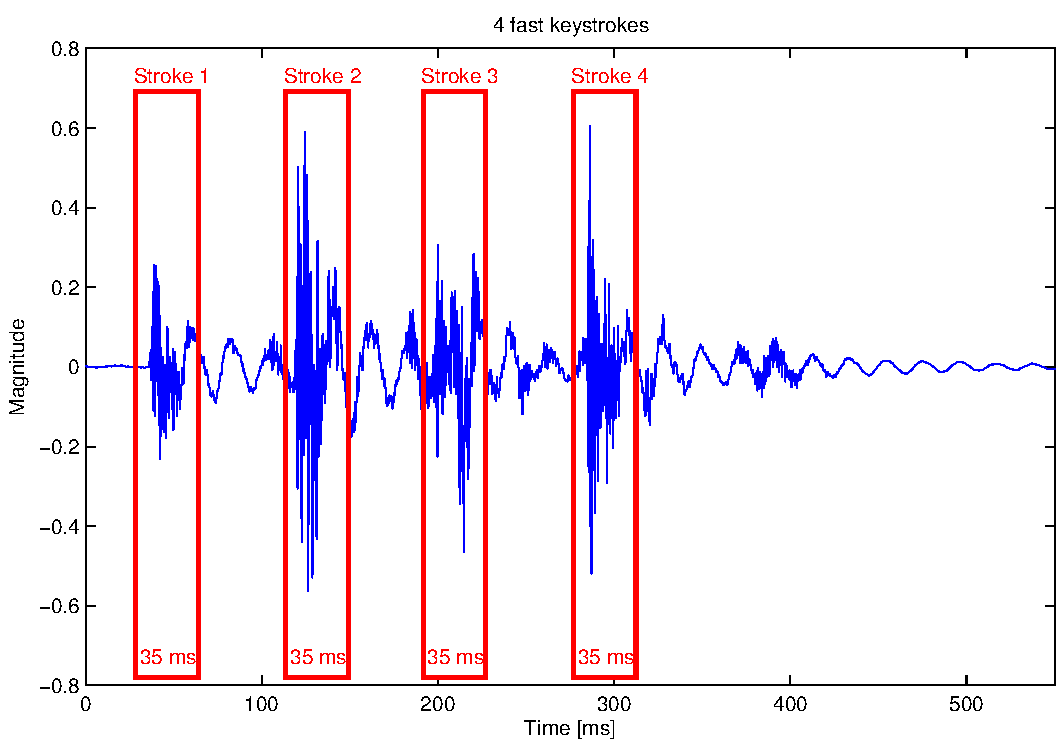
\includegraphics[width=120mm]{Keyboard4StrokesFast.pdf}
\caption{Four annotated keyboard strokes in rapid succession.}\label{fig:Keyboard4StrokesFast}
\end{figure}

\section{Separation pre-filtering}
\section{Noise burst model}
\section{AR filtering approach}

% ------------------------------------------------------------------------


%%% Local Variables:
%%% mode: latex
%%% TeX-master: "../thesis"
%%% End:
